\documentclass[a4paper,12pt]{article} 
\usepackage[T2A]{fontenc}			
\usepackage[utf8]{inputenc}			
\usepackage[english,russian]{babel}	
\usepackage{amsmath,amsfonts,amssymb,amsthm,mathrsfs,mathtools} 
\usepackage{cancel}
\usepackage{multirow}
\usepackage[colorlinks, linkcolor = blue]{hyperref}
\usepackage{upgreek}\usepackage[left=2cm,right=2cm,top=2cm,bottom=3cm,bindingoffset=0cm]{geometry}
\usepackage{tikz}
\usepackage{graphicx}
\usepackage{subfig}
\usepackage{titletoc}
\usepackage{pgfplots}
\usepackage{hhline}
\usepackage{xcolor}
\usepackage{wrapfig}
\newcommand{\angstrom}{\text{\normalfont\AA}}
\author{Дорогинин Д.В.\\
Группа Б02-825}
\title{2.2 и 2.3 Изучение спектров атома водорода и молекулы йода.}
\date{\vspace{-10pt}}

%\begin{wrapfigure}{r}{0.5\textwidth}
%\begin{center}
%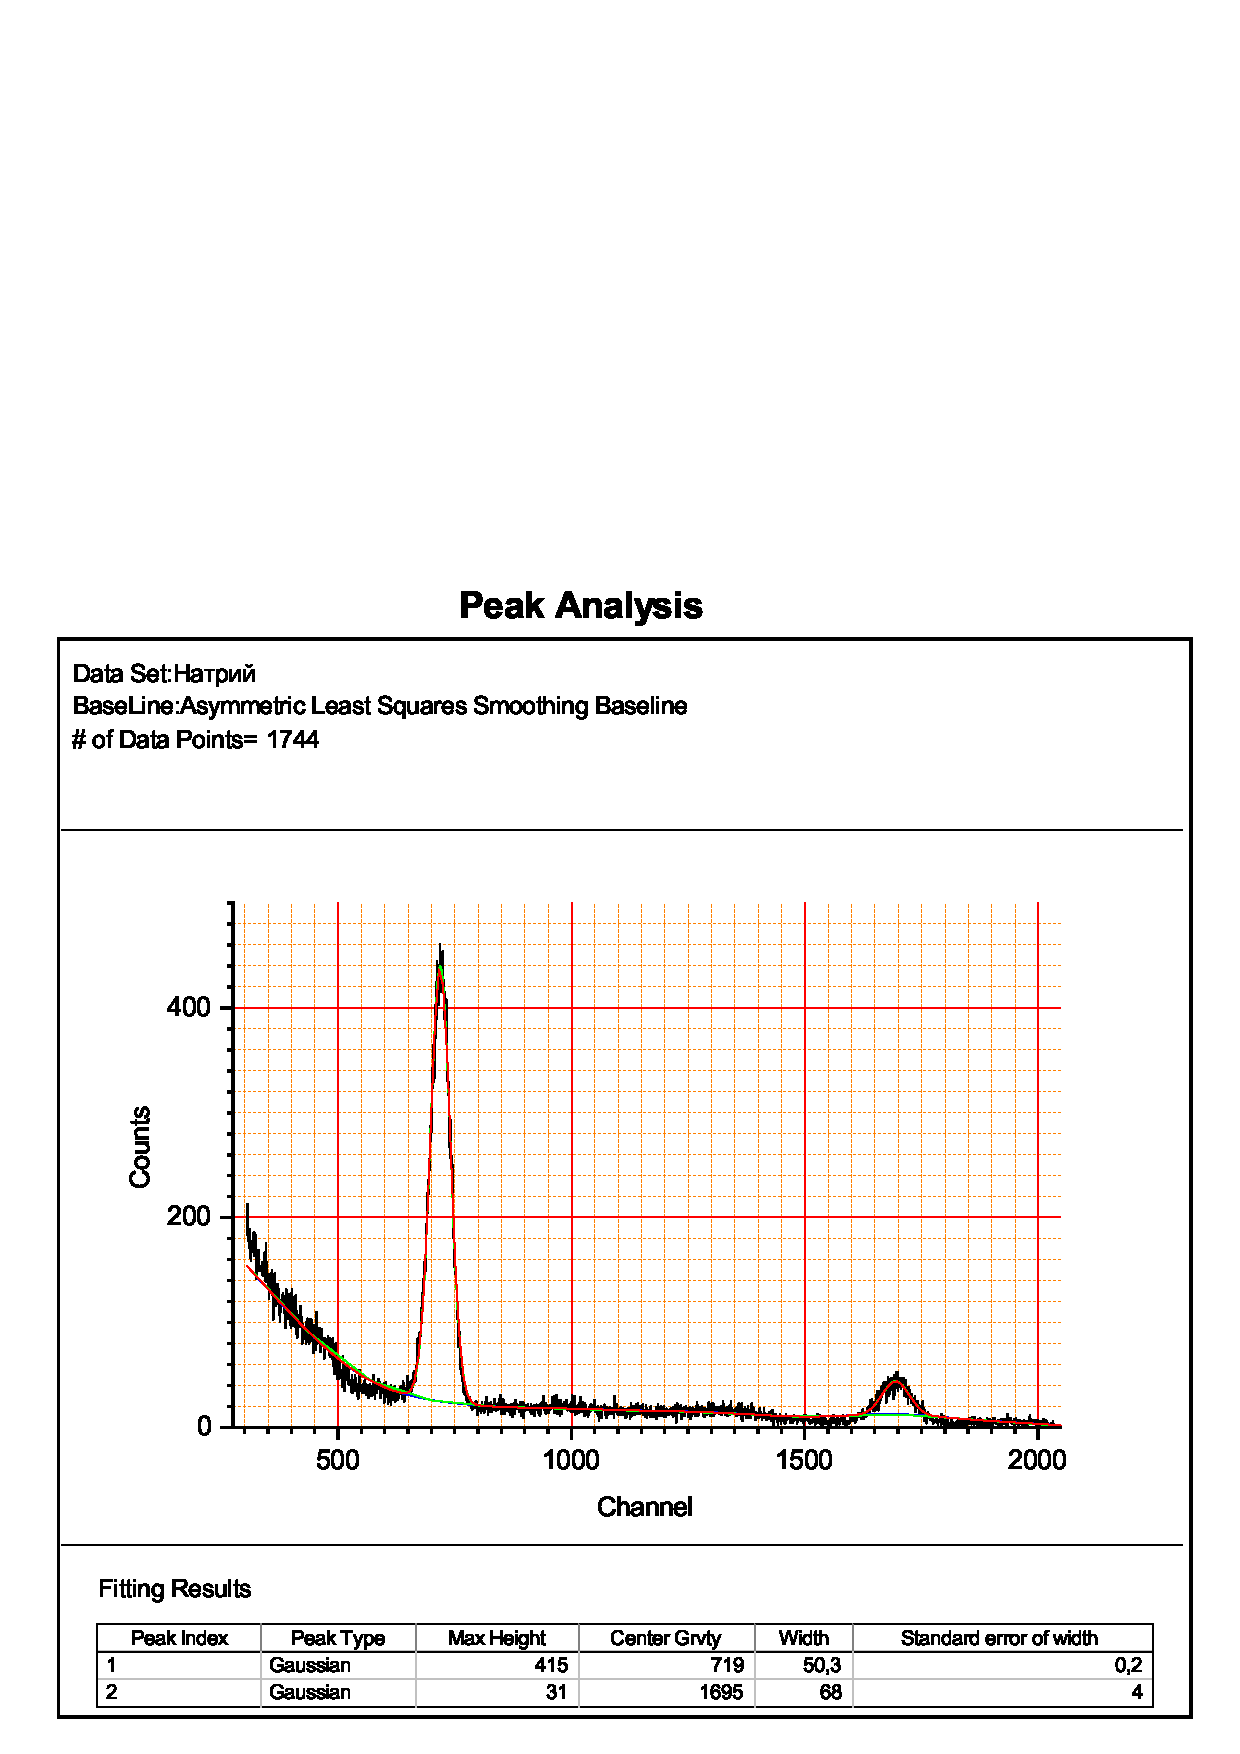
\includegraphics[width = 0.4\textwidth]{1.png}
%\end{center}
%\caption{}
%\end{wrapfigure}

%\begin{wrapfigure}{r}{0.5\textwidth}
%\begin{center}
%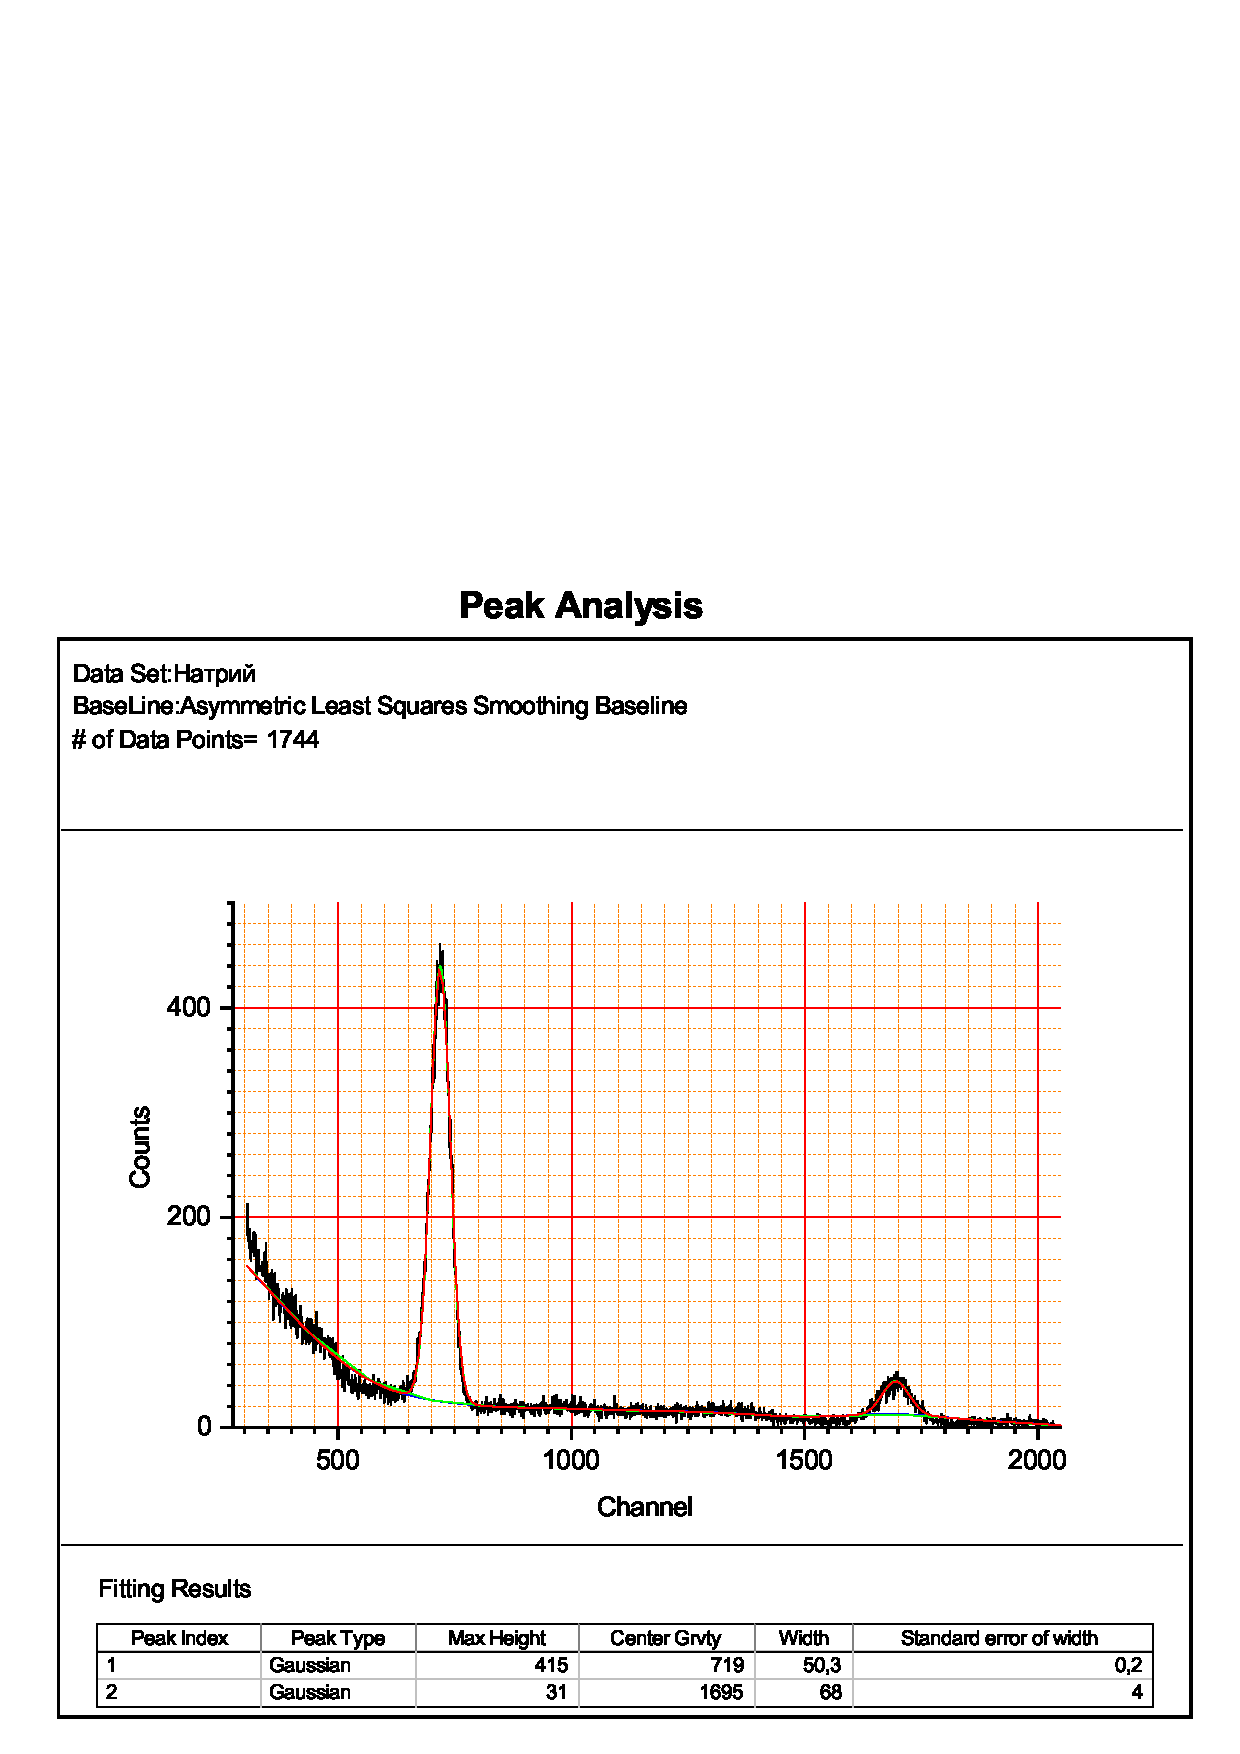
\includegraphics[width = 0.4\textwidth]{1.png}
%\end{center}
%\caption{}
%\end{wrapfigure}

\begin{document}
\maketitle
\textbf{В работе исследуются}: сериальные закономерости в оптическом спектре водорода; спектр поглощения паров йода в видимой области.
\section*{Теория}
Длины волн спектральных линий водородоподобного атома описываются формулой
\begin{equation}
\dfrac{1}{\lambda_{mn}} = RZ^2 \left( \dfrac{1}{n^2} - \dfrac{1}{m^2} \right),
\end{equation}
\begin{wrapfigure}{r}{0.4\textwidth}
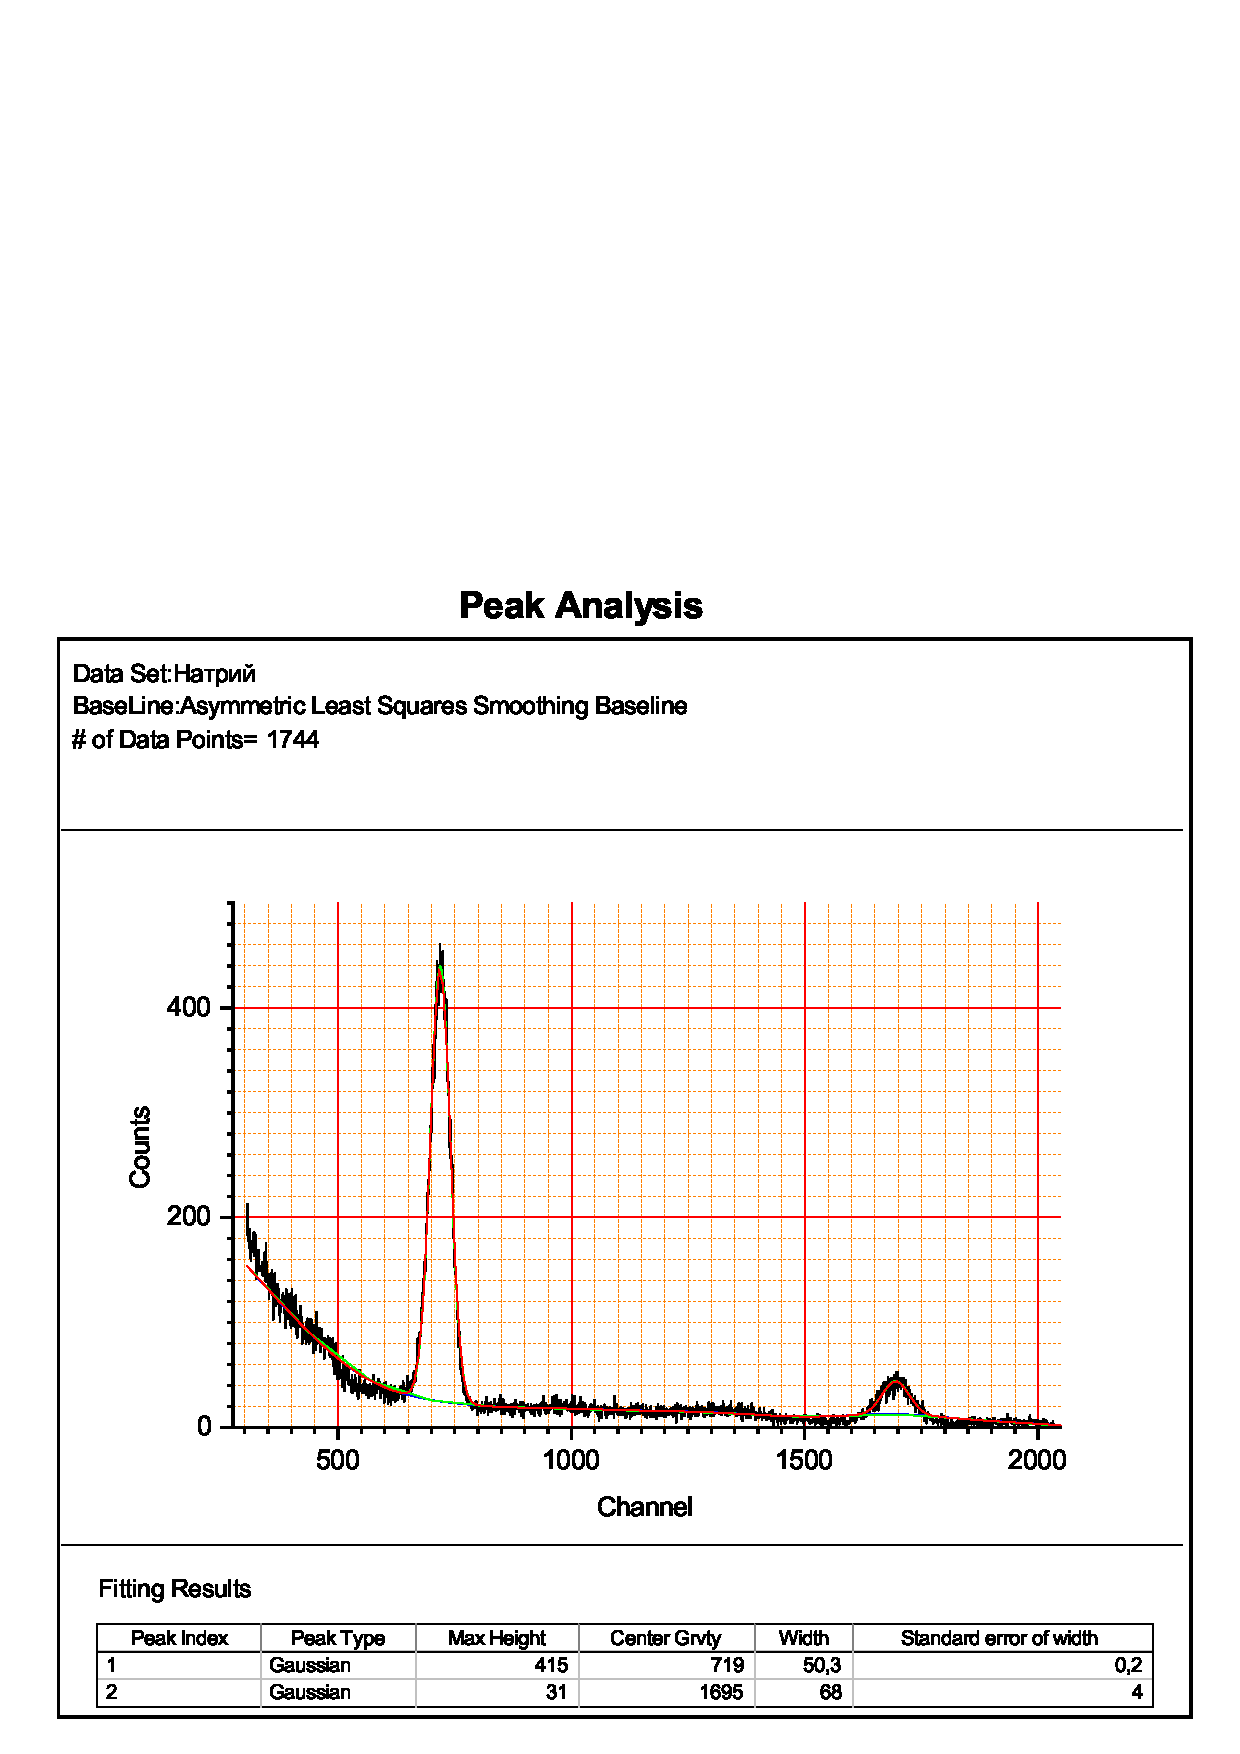
\includegraphics[width = 0.37\textwidth]{1.png}
\centering
\caption{Линии молекулы йода.}
\end{wrapfigure}
где $R = 109677.6~\text{см}^{-1}$ -- константа, называемая постоянной Ридберга, а $m$ и $n$ -- целые числа. Мы будем изучать серию Бальмера, линии которой лежат в видимой области. Для неё $n = 2$, а $m = 3,~4,~5,~6\dots$ Первые четыре линии обозначаются соответственно $H_\alpha$, $H_\beta$, $H_\gamma$, $H_\delta$.
Для молекулы йода мы рассматриваем только нулевую серию, энергетическое положение линий поглощения определяется выражением
\begin{equation}
h\nu_{0, n_2} = (E_2 - E_1) + h\nu_2 \left( n_2 + \dfrac{1}{2} \right) - \dfrac{1}{2} h \nu_1.
\end{equation}
\section*{Описание установки}
Для наблюдения спектра водорода используется установка, изображённая на Рис. 2А. Источником света для наблюдения служит водородная трубка Н-образной формы, в состав газа которой добавлены водные пары для увеличения яркости интересующих нас линий. Источник Л помещается на оптическую скамью вместе с конденсером К, так что свет концентрируется на входной щели 1. Далее через коллиматорный объектив 2 свет попадает на сложную спектральную призму, состояющую из призм П$_1$, П$_2$ и П$_3$. Первые две призмы обладают большой дисперсией, а промежуточная П$_3$ поворачивает лучи -- такое устройство позволяет складывать дисперии П$_1$ и П$_2$. После прохождения призмы свет попадает в зрительную трубу 4-5, объектив которой даёт изображение входной щели различных цветов.
\newpage
\begin{figure}[h]
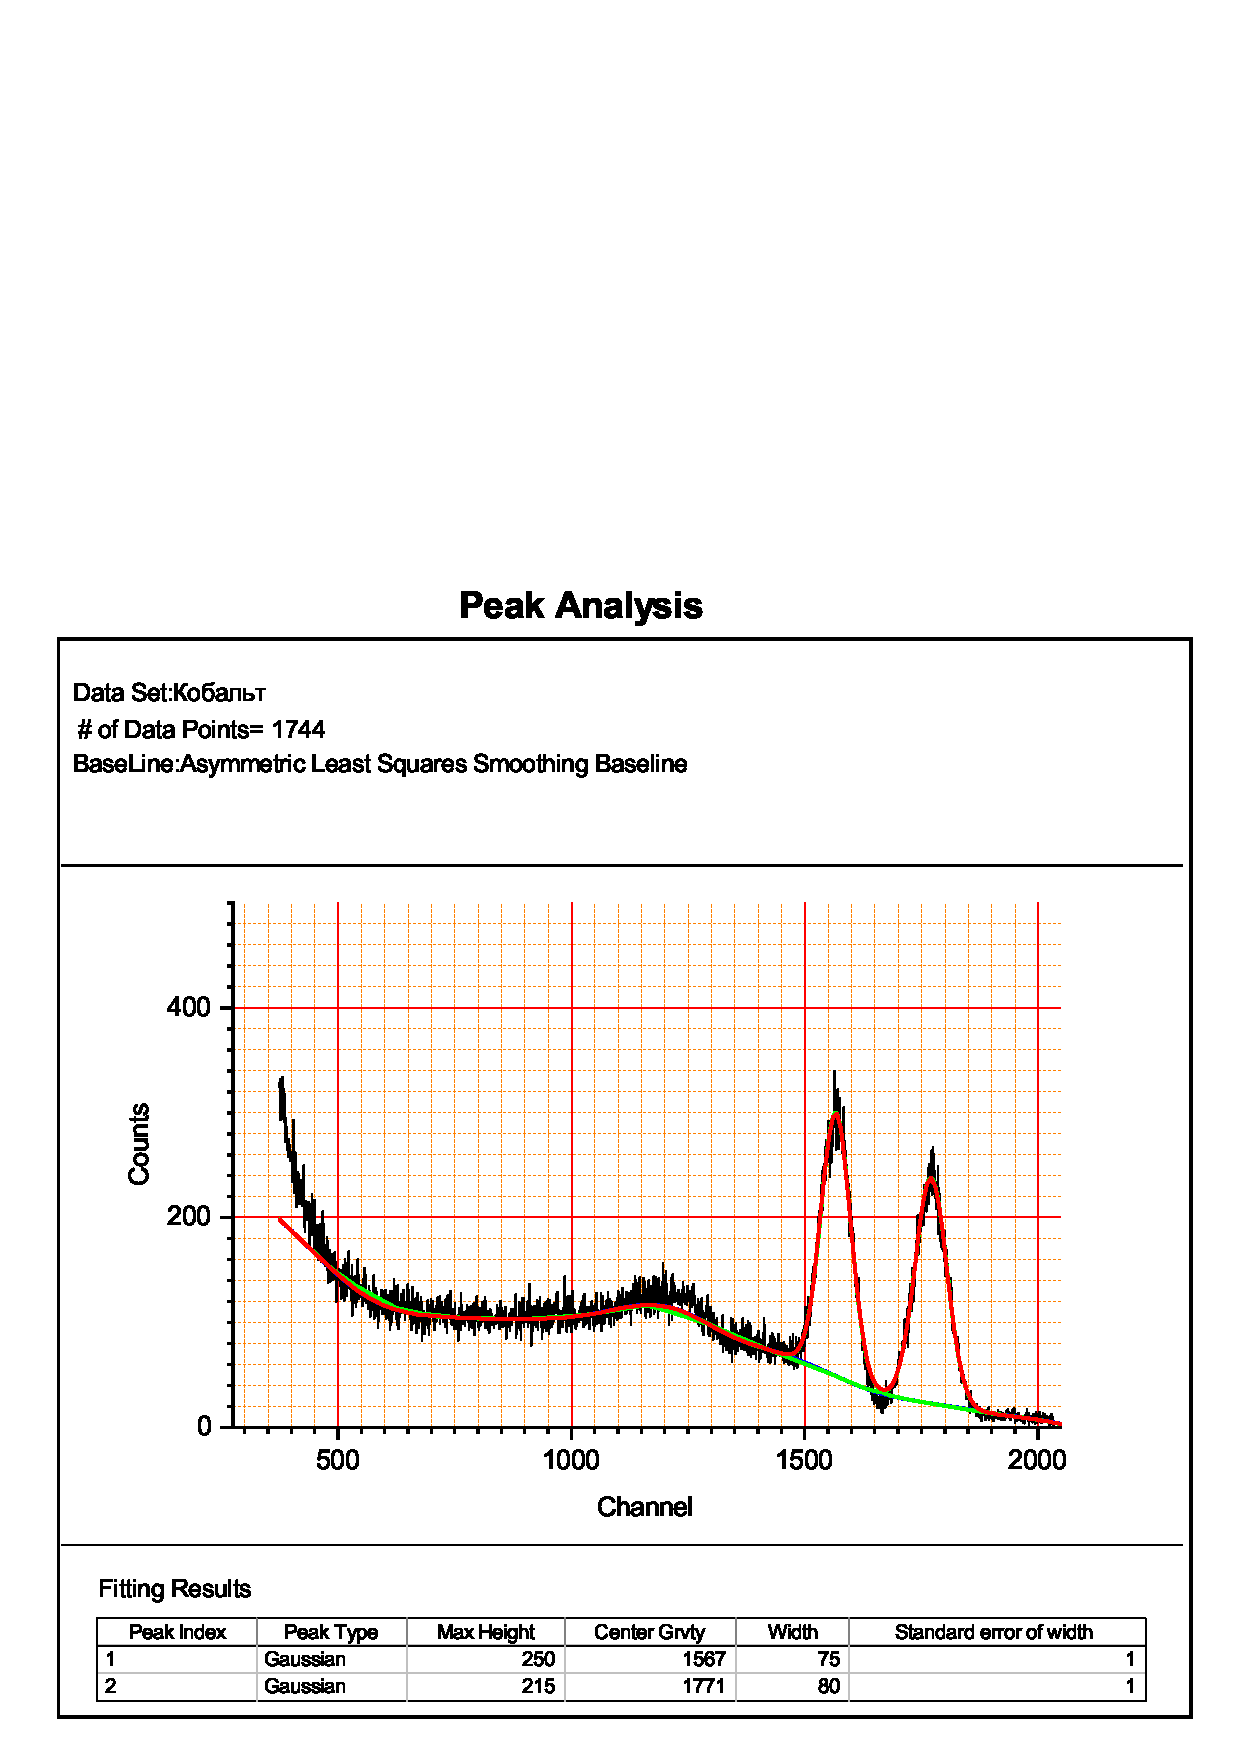
\includegraphics[scale=0.5]{2.png}
\centering
\caption{Установки для наблюдения линий А. водорода; Б. йода.}
\end{figure} 
На Рис. 2Б изображена схема установки, используемой для наблюдения спектра йода. Спектр поглощения паров йода наблюдается визуально на фоне сплошного спектра лампы накаливания 1, питаемой от блока питания 2. Кювета 3 с кристаллами йода подогревается нихромовой спиралью, подключённой вместе с лампой накаливания к блоку питания. Линза 4 используется как конденсор. В результате подогрева кристаллы йода частично возгоняются, образуя пары
с лёгкой фиолетовой окраской. Спектрометр 5 позволяет визуально наблюдать линии поглощения молекул йода на фоне сплошного спектра излучения лампы накаливания видимой области.

\section*{Ход работы}
Сначала произведём градуировку монохроматора. Для этого проведём измерения линий спектра неона и ртути, сняв зависимость длины волны наблюдаемого света $\lambda$ от параметра $\theta$ барабана монохроматора. Погрешность измерения $\theta$ примем половиной цены деления $\sigma_\theta = 5^\circ$. Измерения представлены в Таблице 1.
\begin{table}[h]
\begin{tabular}{|c|c|c|c|c|c|c|c|c|c|}
\hline
$\lambda$, $\angstrom$ & 5401 & 5852 & 5945 & 6030 & 6074 & 6143 & 6217 & 6267 & 6305 \\ \hline
$\theta$, $^\circ$  & 1897 & 2158 & 2204 & 2241 & 2261 & 2292 & 2322 & 2342 & 2356 \\ \hhline{|==========|}
$\lambda$, $\angstrom$ & 6334 & 6383 & 6507 & 6599 & 5791 & 5461 & 4916 & 4358 & 4047 \\ \hline
$\theta$, $^\circ$  & 2368 & 2386 & 2431 & 2466 & 2128 & 1936 & 1515 & 838  & 296  \\ \hline
\end{tabular}
\centering
\caption{Измерения для градуировки.}
\end{table}\\
Искать зависимость $\lambda = \lambda(\theta)$ будем в виде (дисперсионная формула Гартмана):
\[\lambda = \lambda_0 + \dfrac{C}{\theta - \theta_0}.\]
График аппроксимации представлен на Рис. 3, полученные константы:
\[\lambda_0 = 2367 \pm 15~\angstrom,~C = -(607 \pm 6) \cdot 10^4 ~\angstrom,~\theta_0 = 3900^\circ \pm 11^\circ.\]
\newpage
\begin{figure}
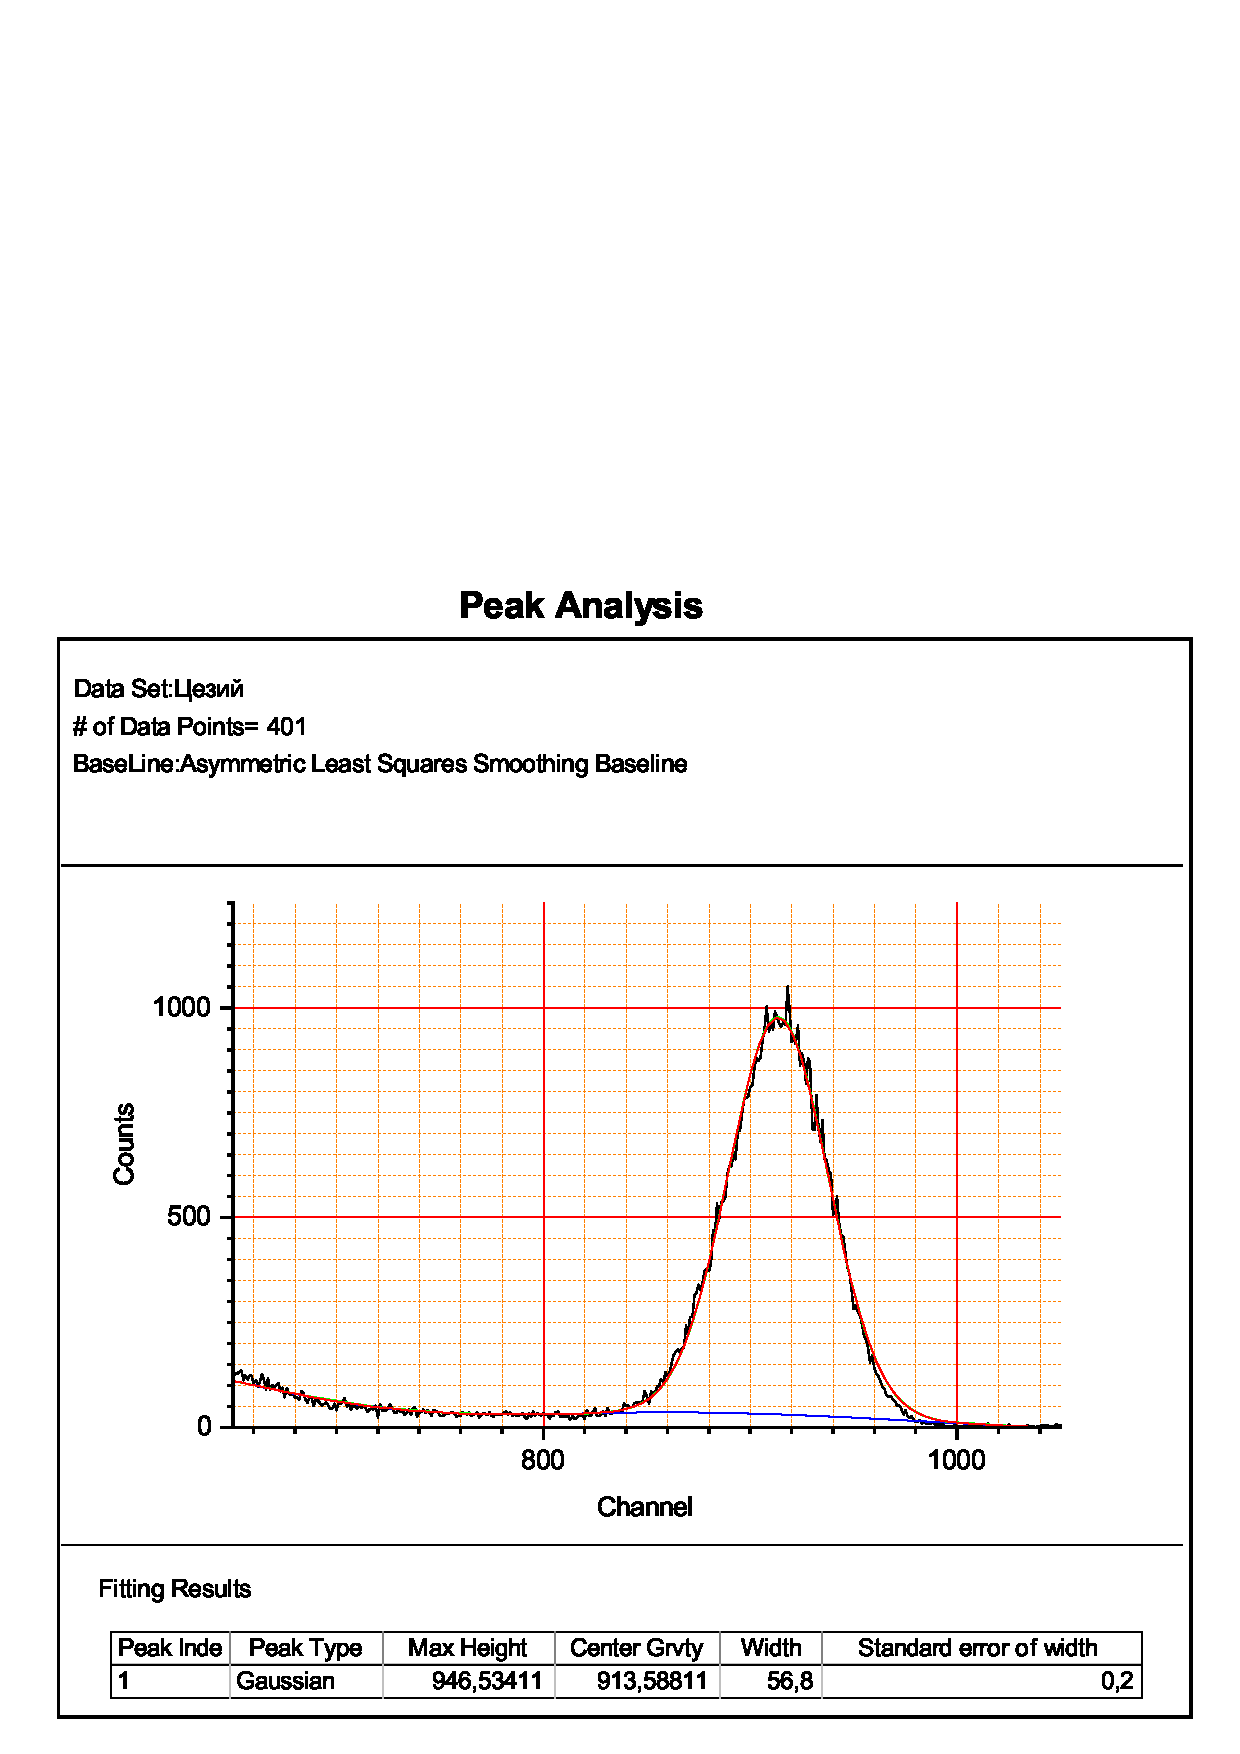
\includegraphics[scale=0.6]{3.png}
\centering
\caption{Зависимость $\lambda = \lambda(\theta)$.}
\end{figure}
Произведём непосредственно измерения для серий водорода. $H_\delta$ у водорода снять не удалось. Измеренные значения параметра барабана для $H_\alpha$, $H_\beta$ и $H_\gamma$:
\[\theta_{32} = 2454^\circ \pm 5^\circ,~\theta_{42} = 1408^\circ \pm 5^\circ,~\theta_{52} = 824^\circ \pm 5^\circ.\]
Соответствующие им длины волн:
\[\lambda_{32} = 656 \pm 3~\text{нм},~\lambda_{42} = 480 \pm 3~\text{нм},~\lambda_{52} = 434 \pm 6~\text{нм}.\]
Воспользовавшись формулой (1), рассчитаем константу Ридберга для каждой из линий, итоговое значение:
\[R = 110100 \pm 800~\text{см}^{-1}.\]
Перейдём к измерениям для йода. Параметры, соответствующие самой длинноволновой линии, линии, отстоящей от неё на 6, и границе спектра:
\[\theta_{1,0} = 2160^\circ \pm 5^\circ,~\theta_{1,5} = 2056^\circ \pm 5^\circ,~\theta_{\text{гр}} = 1722^\circ \pm 5^\circ.\]
Тогда длины волн
\[\lambda_{1,0} = 586 \pm 3~\text{нм},~\lambda_{1,5} = 566 \pm 3~\text{нм},~\lambda_{\text{гр}} = 515 \pm 3~\text{нм}.\]
Энергии колебательного кванта возбуждённого состояния молекулы йода:
\[h\nu_{2} = \dfrac{h\nu_{1,5} - h\nu_{1,0}}{2} = 0.03 \pm 0.02~\text{эВ}.\]
Учитывая, что $h\nu_1 = 0.027~\text{эВ}$, с помощью формулы (2) рассчитаем энергию перехода
\[h\nu_{\text{эл}} = h\nu_{(1,0)} - \dfrac{1}{2} h\nu_2 + \dfrac{3}{2} h\nu_1 = 2.14 \pm 0.03~\text{эВ}.\]
Тогда энергии диссоциации частиц в основном и возбуждённом состоянии, с учётом того, что энергия возбуждения атома $E_A = 0.94~\text{эВ}$:
\[D_1 = h\nu_{\text{гр}} - E_A = 1.47 \pm 0.02~\text{эВ},\]
\[D_2 = h\nu_{\text{гр}} - h\nu_{\text{эл}} = 0.27 \pm 0.03~\text{эВ}.\]
\end{document}
























































